\documentclass[12pt,letterpaper]{article}
\usepackage{graphicx,textcomp}
\usepackage{natbib}
\usepackage{setspace}
\usepackage{fullpage}
\usepackage{color}
\usepackage[reqno]{amsmath}
\usepackage{amsthm}
\usepackage{fancyvrb}
\usepackage{amssymb,enumerate}
\usepackage[all]{xy}
\usepackage{endnotes}
\usepackage{lscape}
\usepackage{float}
\usepackage{hyperref}

\usepackage{parskip} 
\usepackage{titlesec}
\titlespacing*{\section}{0pt}{3ex plus 1ex minus .2ex}{1.5ex plus .2ex}
\titlespacing*{\subsection}{0pt}{2.5ex plus 1ex minus .2ex}{1ex plus .2ex}

\newtheorem{com}{Comment}
\newtheorem{lem}{Lemma}
\newtheorem{prop}{Proposition}
\newtheorem{thm}{Theorem}
\newtheorem{defn}{Definition}
\newtheorem{cor}{Corollary}
\newtheorem{obs}{Observation}
\newtheorem{hyp}{Hypothesis}

\usepackage{dcolumn}
\usepackage{tikz}
\usetikzlibrary{arrows}
\usepackage{multirow}
\usepackage{xcolor}
\newcolumntype{.}{D{.}{.}{-1}}
\newcolumntype{d}[1]{D{.}{.}{#1}}
\definecolor{light-gray}{gray}{0.65}
\usepackage{url}
\usepackage{listings}

\definecolor{codegreen}{rgb}{0,0.6,0}
\definecolor{codegray}{rgb}{0.5,0.5,0.5}
\definecolor{codepurple}{rgb}{0.58,0,0.82}
\definecolor{backcolour}{rgb}{0.95,0.95,0.92}

\lstdefinestyle{mystyle}{
	backgroundcolor=\color{backcolour},
	commentstyle=\color{codegreen},
	keywordstyle=\color{magenta},
	numberstyle=\tiny\color{codegray},
	stringstyle=\color{codepurple},
	basicstyle=\footnotesize,
	breakatwhitespace=false,
	breaklines=true,
	captionpos=b,
	keepspaces=true,
	numbers=left,
	numbersep=5pt,
	showspaces=false,
	showstringspaces=false,
	showtabs=false,
	tabsize=2
}
\lstset{style=mystyle}
\newcommand{\Sref}[1]{Section~\ref{#1}}

\hypersetup{
	colorlinks=true,
	linkcolor=black,
	filecolor=black,      
	urlcolor=black,
	citecolor=black,
}

\title{\textbf{Final Project}}
\date{\today}
\author{Hanyu Li (ID: 25346841)}

\begin{document}
	
	\maketitle
	
	\tableofcontents
	\newpage 
	
	\section*{Executive summary}
	\addcontentsline{toc}{section}{Executive summary} 
	
	Contemporary society faces significant challenges in the digital age. The Echo Chamber concept and the Filter Bubble theory suggest that online algorithm feeds increasingly trap individuals in closed information loops. This process fosters attitude polarization and reduces generalized trust in strangers. However, as argued by Brown (2002), active information navigation skills are crucial components of modern digital literacy. Specifically, the ability to manage privacy preferences and utilize advanced search functions may help individuals resist algorithmic constraints. Therefore, this analysis tries to explore: can active information navigation skills counteract the echo chamber effect and rebuild social trust?\\
	
	To address this question, this study analyzes 27,026 valid responses from the European Social Survey (ESS Round 10 - 2020), which focuses on democracy and digital social contacts. The analysis uses data visualization to explore three main areas:\\
	
	\begin{itemize}
		\item The distribution of social trust scores among European respondents across different information navigation skill levels.
		\item The tension between offline social meeting frequency, daily internet use time, and their combined effect on social trust.
		\item The big picture: a cross-regional comparison of how information navigation skills change with age in Europe. This section explores potential generational and regional digital skill divides.
	\end{itemize}
	
	Ultimately, this study aims to establish an initial understanding of how digital competencies shape social cohesion across different European regions in a data-driven society.\\
	
	\section*{Data background}
	\addcontentsline{toc}{section}{Data background}
	This study utilizes data from the tenth round of the European Social Survey (ESS Round 10). The ESS is a rigorous cross-national survey organized by the European Research Infrastructure Consortium (ESS ERIC). Data collection for this round took place between September 18, 2020, and September 3, 2022. The survey covers 31 European countries and targets individuals aged 15 and over resident within private households, regardless of their nationality or citizenship. Traditionally, the ESS relies on hour-long, face-to-face interviews to collect data. The Round 10 questionnaire focuses specifically on democracy and digital social contacts.\\
	
	To explore the relationship between information navigation skills and social trust, this analysis selects several key variables from the dataset. The specific variables and their corresponding measurement scales are defined as follows:\\
	
	\begin{itemize}
		\item \textbf{Country} (\textit{cntry}): the respondent's country of residence.
		
		\item \textbf{Year of Birth} (\textit{yrbrn}): the respondent's year of birth to calculate age.
		
		\item \textbf{Social Trust} (\textit{ppltrst}): Measures generalized trust using the question: ``Generally speaking, would you say that most people can be trusted, or that you can't be too careful in dealing with people?'' Responses are scored on an 11-point scale from 0 (``You can't be too careful'') to 10 (``Most people can be trusted'').
		
		\item \textbf{Daily Internet Use Time} (\textit{netustm}): Records the self-reported amount of time spent on the internet on a typical day, measured in minutes.
		
		\item \textbf{Offline Social Meeting} (\textit{sclmeet}): Measures the frequency of meeting socially with friends, relatives, or colleagues.
		
		\item \textbf{Preference Settings Familiarity} (\textit{fampref}): Assesses the respondent's familiarity with managing computer and internet preference settings. Responses range from 1 (``Not at all familiar'') to 5 (``Completely familiar'').
		
		\item \textbf{Advanced Search Familiarity} (\textit{famadvs}): Assesses the respondent's familiarity with utilizing advanced search functions. Responses also range from 1 (``Not at all familiar'') to 5 (``Completely familiar'').
	\end{itemize}
	
	\section*{Data cleaning}
	\addcontentsline{toc}{section}{Data cleaning}
	The data cleaning process was as follows:\\
	First, cases containing missing values, refusals to answer, or invalid entries across key variables were entirely excluded from the dataset to maintain data integrity. Next, survey responses initially stored as character or factor types were converted into proper numeric formats to facilitate accurate mathematical operations. Following this, a new composite variable, \textit{Information Navigation Skill} (\textit{navskill}), was created by calculating the mean score of the respondents' familiarity with preference settings and advanced search functions. Finally, grouping variables, specifically offline social meeting frequency and the newly constructed navigation skill levels, were transformed into ordered factors. This step ensures that categorical data is displayed in a logical hierarchical sequence in the final plots. Through these procedures, a streamlined dataset containing 27,026 valid observations was established, focusing exclusively on the core variables required for analysis.\\
	\lstinputlisting[language=R, firstline=7, lastline=45]{final_project_HL.R}
	
	\begin{verbatim}
		tibble [27,026 x 6] (S3: tbl_df/tbl/data.frame)
		$ cntry      : chr [1:27026] "BE" "BE" "BE" "BE" ...
		$ yrbrn      : num [1:27026] 2006 1998 1964 1987 1961 ...
		$ ppltrst    : num [1:27026] 6 3 6 7 3 4 6 7 3 3 ...
		$ netustm    : num [1:27026] 8 240 120 90 120 120 10 180 210 120 ...
		$ social_freq: Factor w/ 7 levels "Never","Less than once a month",..: 5 4 4 5 6 6 4 6 5 4 ...
		$ navskill   : Factor w/ 5 levels "Very Low","Low",..: 3 5 3 1 3 4 5 4 3 5 .
	\end{verbatim} 
	
	\section*{Individual figures}
	\addcontentsline{toc}{section}{Individual figures}
	
	\subsection*{Figure 1: Distribution of Social Trust by Information Navigation Skills}
	\addcontentsline{toc}{subsection}{Figure 1: Distribution of Social Trust by Information Navigation Skills}
	To address the primary research question, I first explored how social trust scores are distributed across different levels of information navigation skills. Figure 1 utilizes a ridge plot to visualize these distributions, where the color gradient from light blue to dark navy represents the progression of skill levels from "Very Low" to "Very High," and the orange points indicate the average social trust score for each group. Visually, as navigation skill levels increase, both the density curves and the mean scores consistently shift toward the higher end of the 0-10 scale. This indicates a positive correspondence between higher digital navigation skills and greater generalized social trust among respondents.\\
	\lstinputlisting[language=R, firstline=66, lastline=99]{final_project_HL.R}
	
	\begin{figure}[H]
		\centering
		
\includegraphics[width=1\textwidth]{plot1.pdf}
	\end{figure}
	
	\subsection*{Figure 2: Social Trust by Internet Use and Social Frequency}
	\addcontentsline{toc}{subsection}{Figure 2: Social Trust by Internet Use and Social Frequency}
	Building upon the observation from Figure 1 that higher information navigation skills correspond with increased social trust, I aimed to further explore the interplay between respondents' online and offline activities. Thus, I investigated the relationship between daily internet use time, offline social meeting frequency, and average social trust scores. My goal was to examine whether these online and offline dimensions exhibit tension or mutually moderate each other.\\
	I found that higher frequencies of offline social interaction are associated with higher baseline levels of social trust. However, I noticed an interesting divergence among individuals who engage in offline social meetings "Every day." For this highly sociable group, as their daily internet use time increases, particularly beyond 4 to 6 hours, their average social trust score notably declines. In contrast, groups with less frequent social meetings maintain a relatively flatter trajectory. I note that this specific phenomenon, where extensive online exposure appears to counter the positive association of daily offline socialization with trust, visually aligns with theoretical perspectives concerning digital saturation and the potential for prolonged online engagement to disrupt real-world social capital.
	\lstinputlisting[language=R, firstline=103, lastline=156]{final_project_HL.R}
	\begin{figure}[H]
		\centering
		
\includegraphics[width=1\textwidth]{plot2.pdf}
	\end{figure}
	
	\subsection*{Figure 3a: Information Navigation Skills Across European Regions}
	\addcontentsline{toc}{subsection}{Figure 3a: Information Navigation Skills Across European Regions}
	After understanding the micro-level perspective of individuals, I aimed to examine the digital issue from a more macro perspective through cross-regional and longitudinal comparisons. Therefore, I first categorized the 31 surveyed countries into four geographic regions: Nordic Countries, Western Europe, Southern Europe, and Central \& Eastern Europe.\\
	Then I visualized the smoothed proportion of information navigation skill levels across the continuous age range to perform a cross-regional comparison.\\ Figure 3a illustrates a universal trend: as age increases, all regions experience a decline in information navigation capabilities, marked by the shrinking of dark blue areas (high skills). However, the rate of decline and the inflection points differ significantly across regions. For instance, the Nordic Countries demonstrate certain digital resilience: even at the age of 50, the combined proportion of 'High' and 'Very High' skills still accounts for approximately 50\%. In contrast, Southern Europe and Central \& Eastern Europe exhibit a much earlier and faster decline. In these regions, the lower-skill categories (lighter blue colors) rapidly expand and become the overwhelming majority for respondents over the age of 40, visually highlighting a severe regional digital divide.
	\lstinputlisting[language=R, firstline=159, lastline=201]{final_project_HL.R}
	\begin{figure}[H]
		\centering
		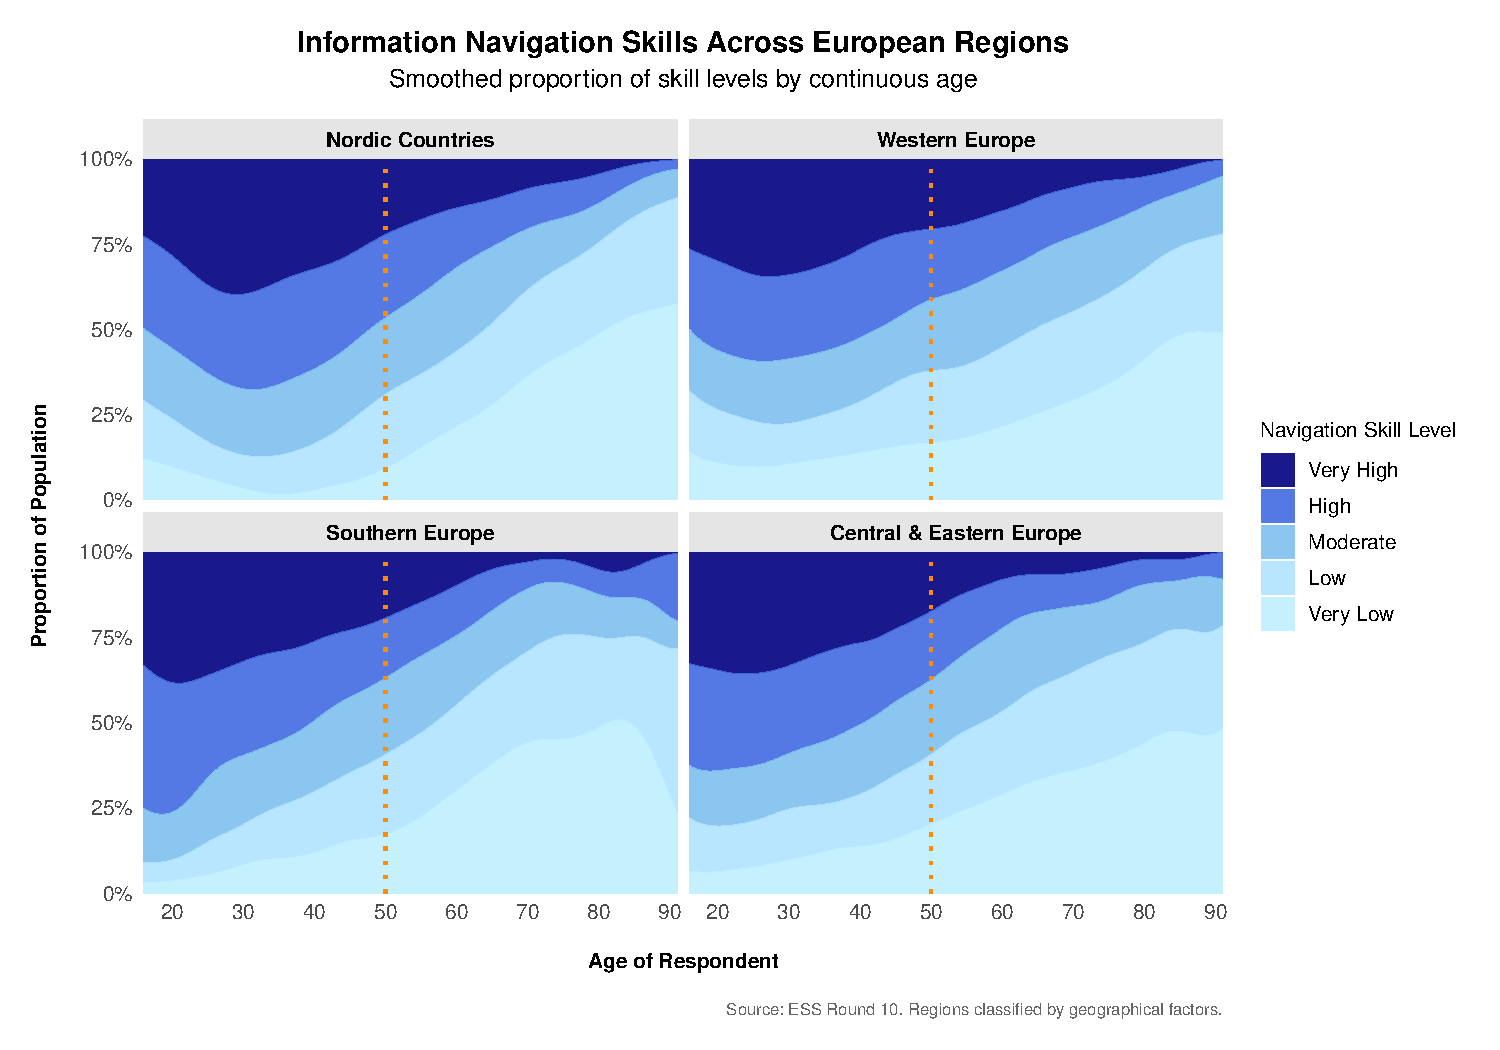
\includegraphics[width=1\textwidth]{plot3a.pdf}
	\end{figure}
	
	
	\subsection*{Figure 3b: Regional Comparison of Information Navigation Skill Decline}
	\addcontentsline{toc}{subsection}{Figure 3b: Regional Comparison of Information Navigation Skill Decline}
	To achieve a sharper and more focused comparison, I isolated and combined the "High" and "Very High" categories into a single high-proficiency group in Figure 3b and I applied a LOESS smoothing model to trace this group's proportion across the age spectrum and explicitly marked the peak and trough values for each European region. \\
	The results present an interesting contrast to the broader trends observed previously. While the Nordic Countries and Western Europe display a relatively smooth overall skill transition across age cohorts, Figure 3b reveals that their absolute drop in top-tier information navigation proficiency is actually the most drastic, plummeting by roughly 60\% to 70\% from youth to old age. Conversely, Southern Europe and Central \& Eastern Europe experience a rapid early decline, yet their lowest high-skill proportions stabilize at a floor of around 20\%. \\
	Most notably, Southern Europe even exhibits an unexpected upward trend in high-skill group proportion after the age of 70. This counter-intuitive rebound, alongside the stable 20\% floor, might suggest a demographic survivorship effect that the elderly respondents accessible and willing to complete the survey inherently have a certain level of digital literacy. Alternatively, it may indicate that a specific subset of the elderly population in these regions maintains active digital engagement, possibly facilitated by strong intergenerational family support structures or targeted digital inclusion initiatives.
	\lstinputlisting[language=R, firstline=205, lastline=272]{final_project_HL.R}
	
	\begin{figure}[H]
		\centering
		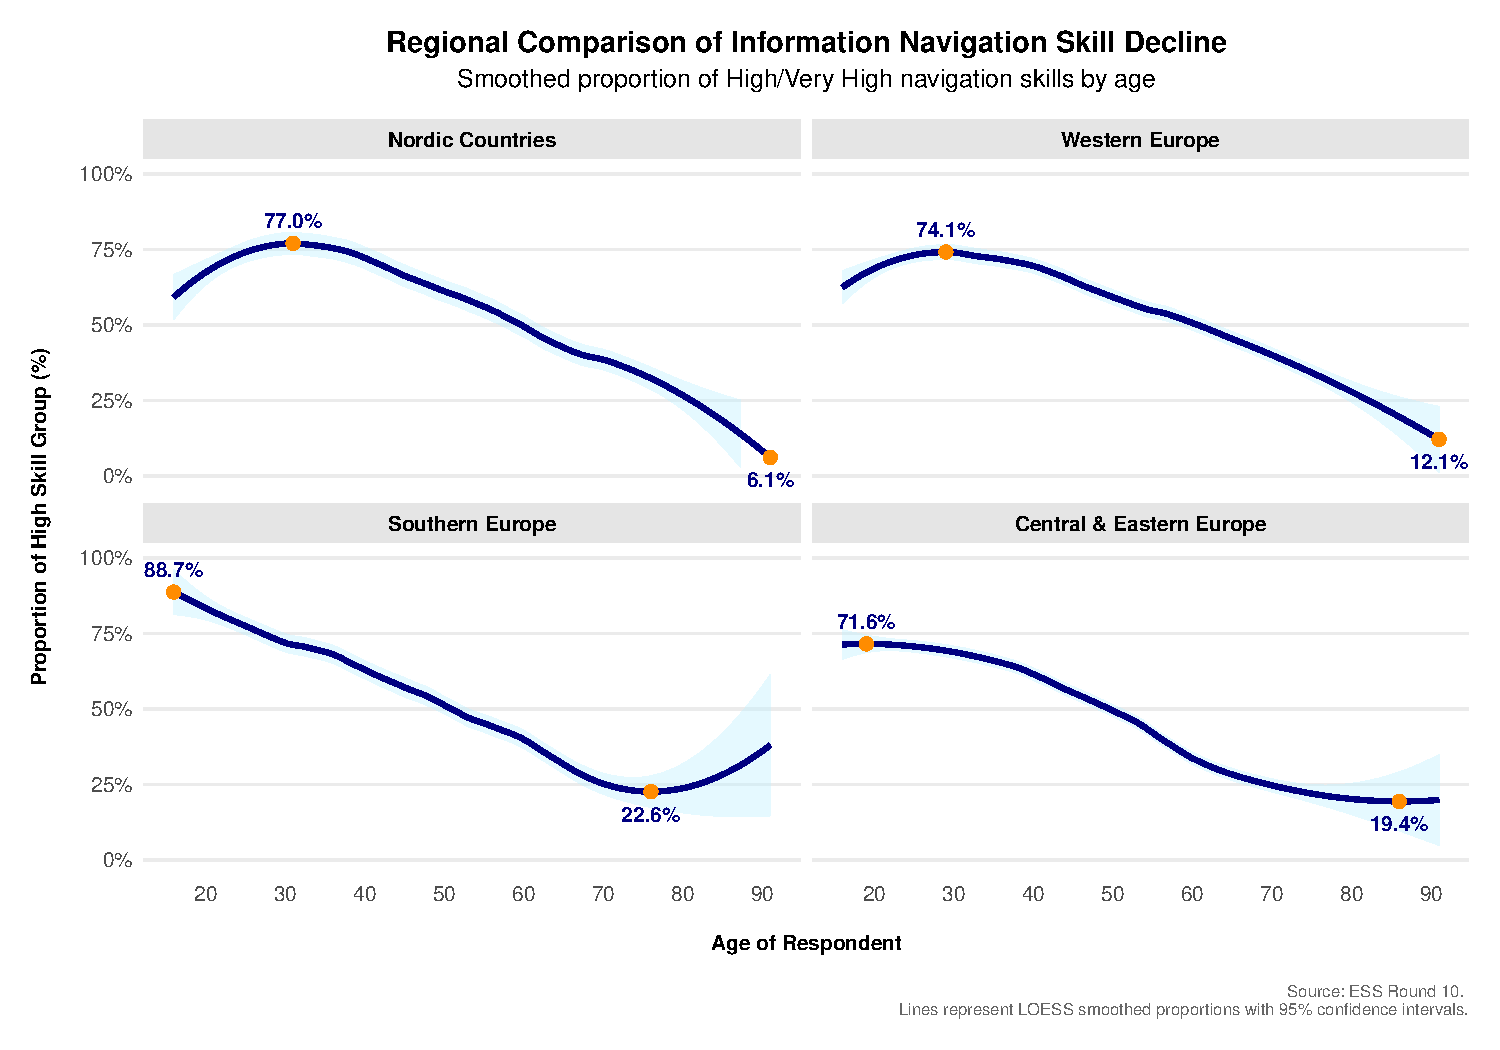
\includegraphics[width=1\textwidth]{plot3b.pdf}
	\end{figure}
	
\end{document}